%!TEX root = ../dissertation.tex
\chapter{Introduction}
\label{introduction}

\newthought{Liquid hydrocarbons are a crucial part} of the modern world's infrastructure. These energy-dense chemicals make up the fuels that power our homes and vehicles, and are the basis of plastics, industrial chemicals and synthetic materials \cite{Refworks:27}. Typically, hydrocarbons are refined from nonrenewable, environmentally harmful sources such as natural gas and crude oil. A practical renewable source of hydrocarbons would therefore reduce our dependence on fossil fuels and constitute a major milestone on the path to overall environmental sustainability \cite{RefWorks:28}.

A prime candidate for this source is cellulose, the carbohydrate polymer that makes up the majority of plant matter \cite{RefWorks:29}. It is the most abundant organic compound on the planet, and it is capable of being transformed into an array of useful chemicals, including ethanol \cite{RefWorks:30}. However, current conversion methods fail to be cost-effective. Chemical and enzymatic depolymerization approaches are generally slow and expensive, while faster pyrolytic methods lack precise product output and generate significant amounts of solid and gaseous waste \cite{RefWorks:30}. The ideal conversion process would have the speed of pyrolysis and the precise efficiency of enzymatic processing.

\begin{figure}
	\centering
	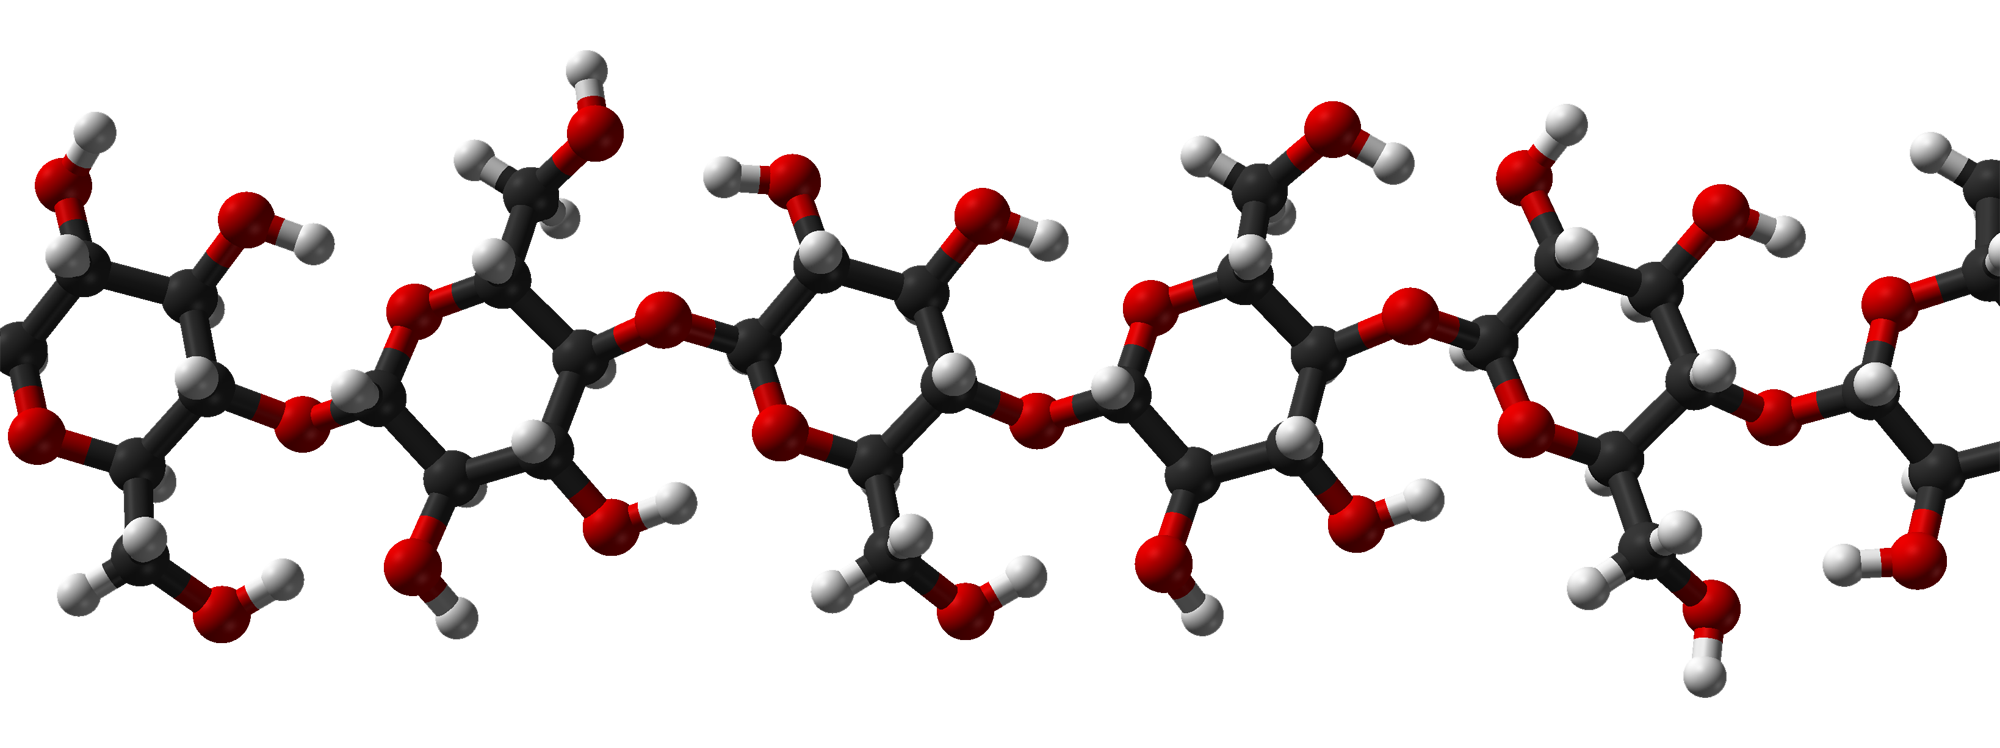
\includegraphics[width=0.7\linewidth]{Cellulose-structure}
	\caption{A visualization of a single cellulose strand.}
	\label{fig:Cellulose-structure}
\end{figure}

To develop such a process, a greater understanding of cellulose pyrolysis is needed. In the interest of developing this understanding, we have studied the effects of increasing temperature on the vibrational spectra of cellobiose, the glucose dimer that makes up cellulose. These spectra reveal the structure and behavior of the molecule, and by investigating them both experimentally and via simulation we have improved our understanding of how heat interacts with cellulose.

\section{Theory}

\subsection{Vibrational Spectroscopy}

As its name suggests, vibrational spectroscopy is predicated on the vibrations of molecules. These vibrations affect a molecule's properties, which in turn affect how it interacts with light. We can exploit these phenomena by illuminating molecules with carefully controlled light and examining the spectrum of frequencies that are reflected. This spectrum encodes information about the underlying molecular vibrations, and thus about the nature of the molecule itself.

A mathematical description of vibration begins with the concept of \emph{degrees of freedom}. The state of any molecule is described by that molecule's degrees of freedom, which enumerate the number of meaningful ways in which the molecule's structure may vary. A single atom has three degrees of freedom, since it may move independently in three spatial directions. A linear molecule composed of two bonded atoms has the same three degrees of freedom, as well as two rotational degrees of freedom, which are axes about which the molecule can spin. Finally, it has one \emph{vibrational} degree of freedom, since the length of the bond may vary, bringing the total number of degrees of freedom to 6. For larger, non-linear molecules, a third axis of rotation becomes available, and the number of vibrational degrees of freedom increases. In general, a molecule with $N$ atoms will have $3N$ degrees of freedom, with three describing overall translations of the molecule and three describing overall rotations, bringing the number of vibrational degrees of freedom to $3N-6$. For each of these degrees there is an associated quantized vibrational energy. The extent of the vibration is determined by the energy level, and each particular vibration can absorb energy quanta energy to transition to a higher level or emit energy quanta to transition to a lower level.

\begin{figure}
	\centering
	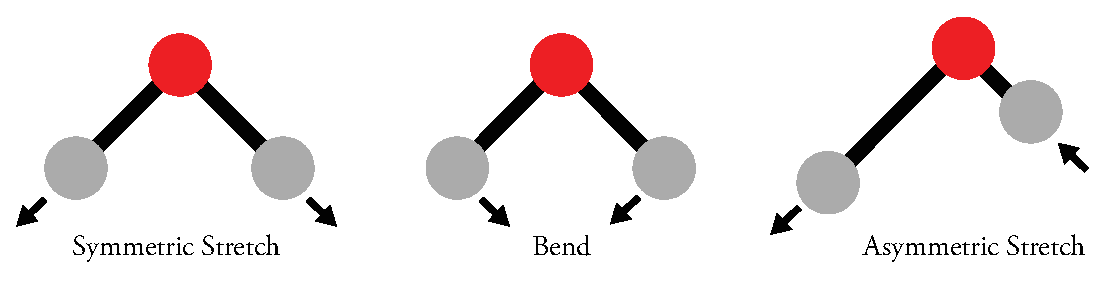
\includegraphics[width=0.7\linewidth]{deg_freedom}
	\caption{The vibrational modes of water.}
	\label{fig:deg_freedom}
\end{figure}

As an example, vibrational degrees of freedom for water are illustrated in Figure \ref{fig:deg_freedom}. They include ``stretch'' motions, which involve changing bond lengths, and a ``bend'' which changes bond angle. These motions, also referred to as \emph{vibrational modes,} represent a complete basis for describing the deformations of a water molecule. Any complicated vibration can be described as a linear combination of these motions.

As a molecule vibrates, its physical and chemical properties fluctuate as well. For example, as the water molecule undergoes the symmetric stretch depicted above, the charges held by its atoms go from being relatively concentrated to relatively separated. This amounts to a change in the molecule's dipole moment. Another property that varies in this way is the molecule's polarizability; in general, the shape of the molecule's charge cloud determines how easy the molecule is to polarize, and since vibrations deform this cloud, they change the polarizability.

Before we begin a mathematical treatment of the subject, a note on units: spectroscopists typically measure frequency in wavenumbers, the number of full wave cycles completed per unit distance. Therefore it is common to see frequency reported in inverse centimeters. with this in mind, consider some arbitrary vibrational mode of a cellobiose molecule with a characteristic frequency $\nu_{\mathrm{vib}}$. When this mode is in its equilibrium position, the molecule has polarizability $\alpha_0$, but as the vibration proceeds, the instantaneous polarizability changes. We can write this as
\begin{equation}
\alpha (t) = \alpha_0 + \beta\sin(2\pi\nu_\mathrm{vib} t)
\end{equation}

where $\beta$ is a constant describing the strength of this vibration's effect on polarizability. A similar equation can be written describing the molecule's osciallating dipole moment.

Now consider a beam of light incident on the molecule. This beam is an oscillating electric field $E$ with a strength $E_0$ and a frequency $\nu$:
\begin{equation}
E = E_0\sin(2\pi\nu t)
\end{equation}
The molecule is polarizable; therefore, in the prescence of this electric field it will have a time-varying induced dipole $\mu$ determined by the equation
\begin{equation}
\label{eq:simple_dipole}
\mu = \alpha E_0\sin(2\pi\nu t)
\end{equation}
This oscillating dipole will emit radiation at frequency $\nu$. In other words, shining light of some frequency on the molecule will cause light of the same frequency to be reflected. Physically, this amounts to elastic scattering of photons off of the molecule, a phenomenon known as Rayleigh scattering.

For a static molecule this would be the end of the story. However, since the molecule is vibrating, Equation \ref{eq:simple_dipole} is incomplete. We must include the time-varying polarizability:

\begin{align}
\mu &= \left[\alpha_0 + \beta\sin(2\pi\nu_\mathrm{vib} t)\right] \cdot E_0\sin(2\pi\nu t)\\
&= \alpha_0E_0\sin(2\pi\nu t) + \beta E_0\sin(2\pi\nu_\mathrm{vib}t)\sin(2\pi\nu t)\\
&= \alpha_0E_0\sin(2\pi\nu t) + \frac{1}{2}\beta E_0\left[\cos(2\pi(\nu - \nu_\mathrm{vib})t) - \cos(2\pi(\nu + \nu_\mathrm{vib})t)\right]
\end{align}

The result shows that the molecule will radiate at not one but three frequencies: $\nu$, $\nu + \nu_\mathrm{vib}$, and  $\nu - \nu_\mathrm{vib}$. These frequencies will be observed if the polarizability of the molecule changes as it vibrates, and the intensity of the radiation will be proportional to $\beta$, the strength of the vibration's effect on the polarizability\cite{RefWorks:31}.

This radiation was predicted by Indian physicist C.V. Raman in 1922, and in his honor it is referred to as Raman radiation. Though we have so far framed this discussion by considering light as a wave, on a deeper level the physics are due to the quantum nature of light and energy. We observe Raman radiation because of inelastic scattering of photons, a phenomenon known as the Raman effect.

Most photons incident on an atom are reflected or scattered elastically: they interact with an atom which is in a ground state, and though the atom may increase in energy during this interaction, the atom returns to its ground state as the interaction finishes. By conservation of energy, the photon must exit with an unchanged energy (and hence frequency) as well. As mentioned above, this is Rayleigh scattering. However, in a small fraction of cases (as small as one in ten million), the photon interacts with an atom that returns to an energy state higher or lower than its original state. The energy difference is transferred to the photon, which is scattered with a shifted frequency.

\begin{figure}[h]
\centering
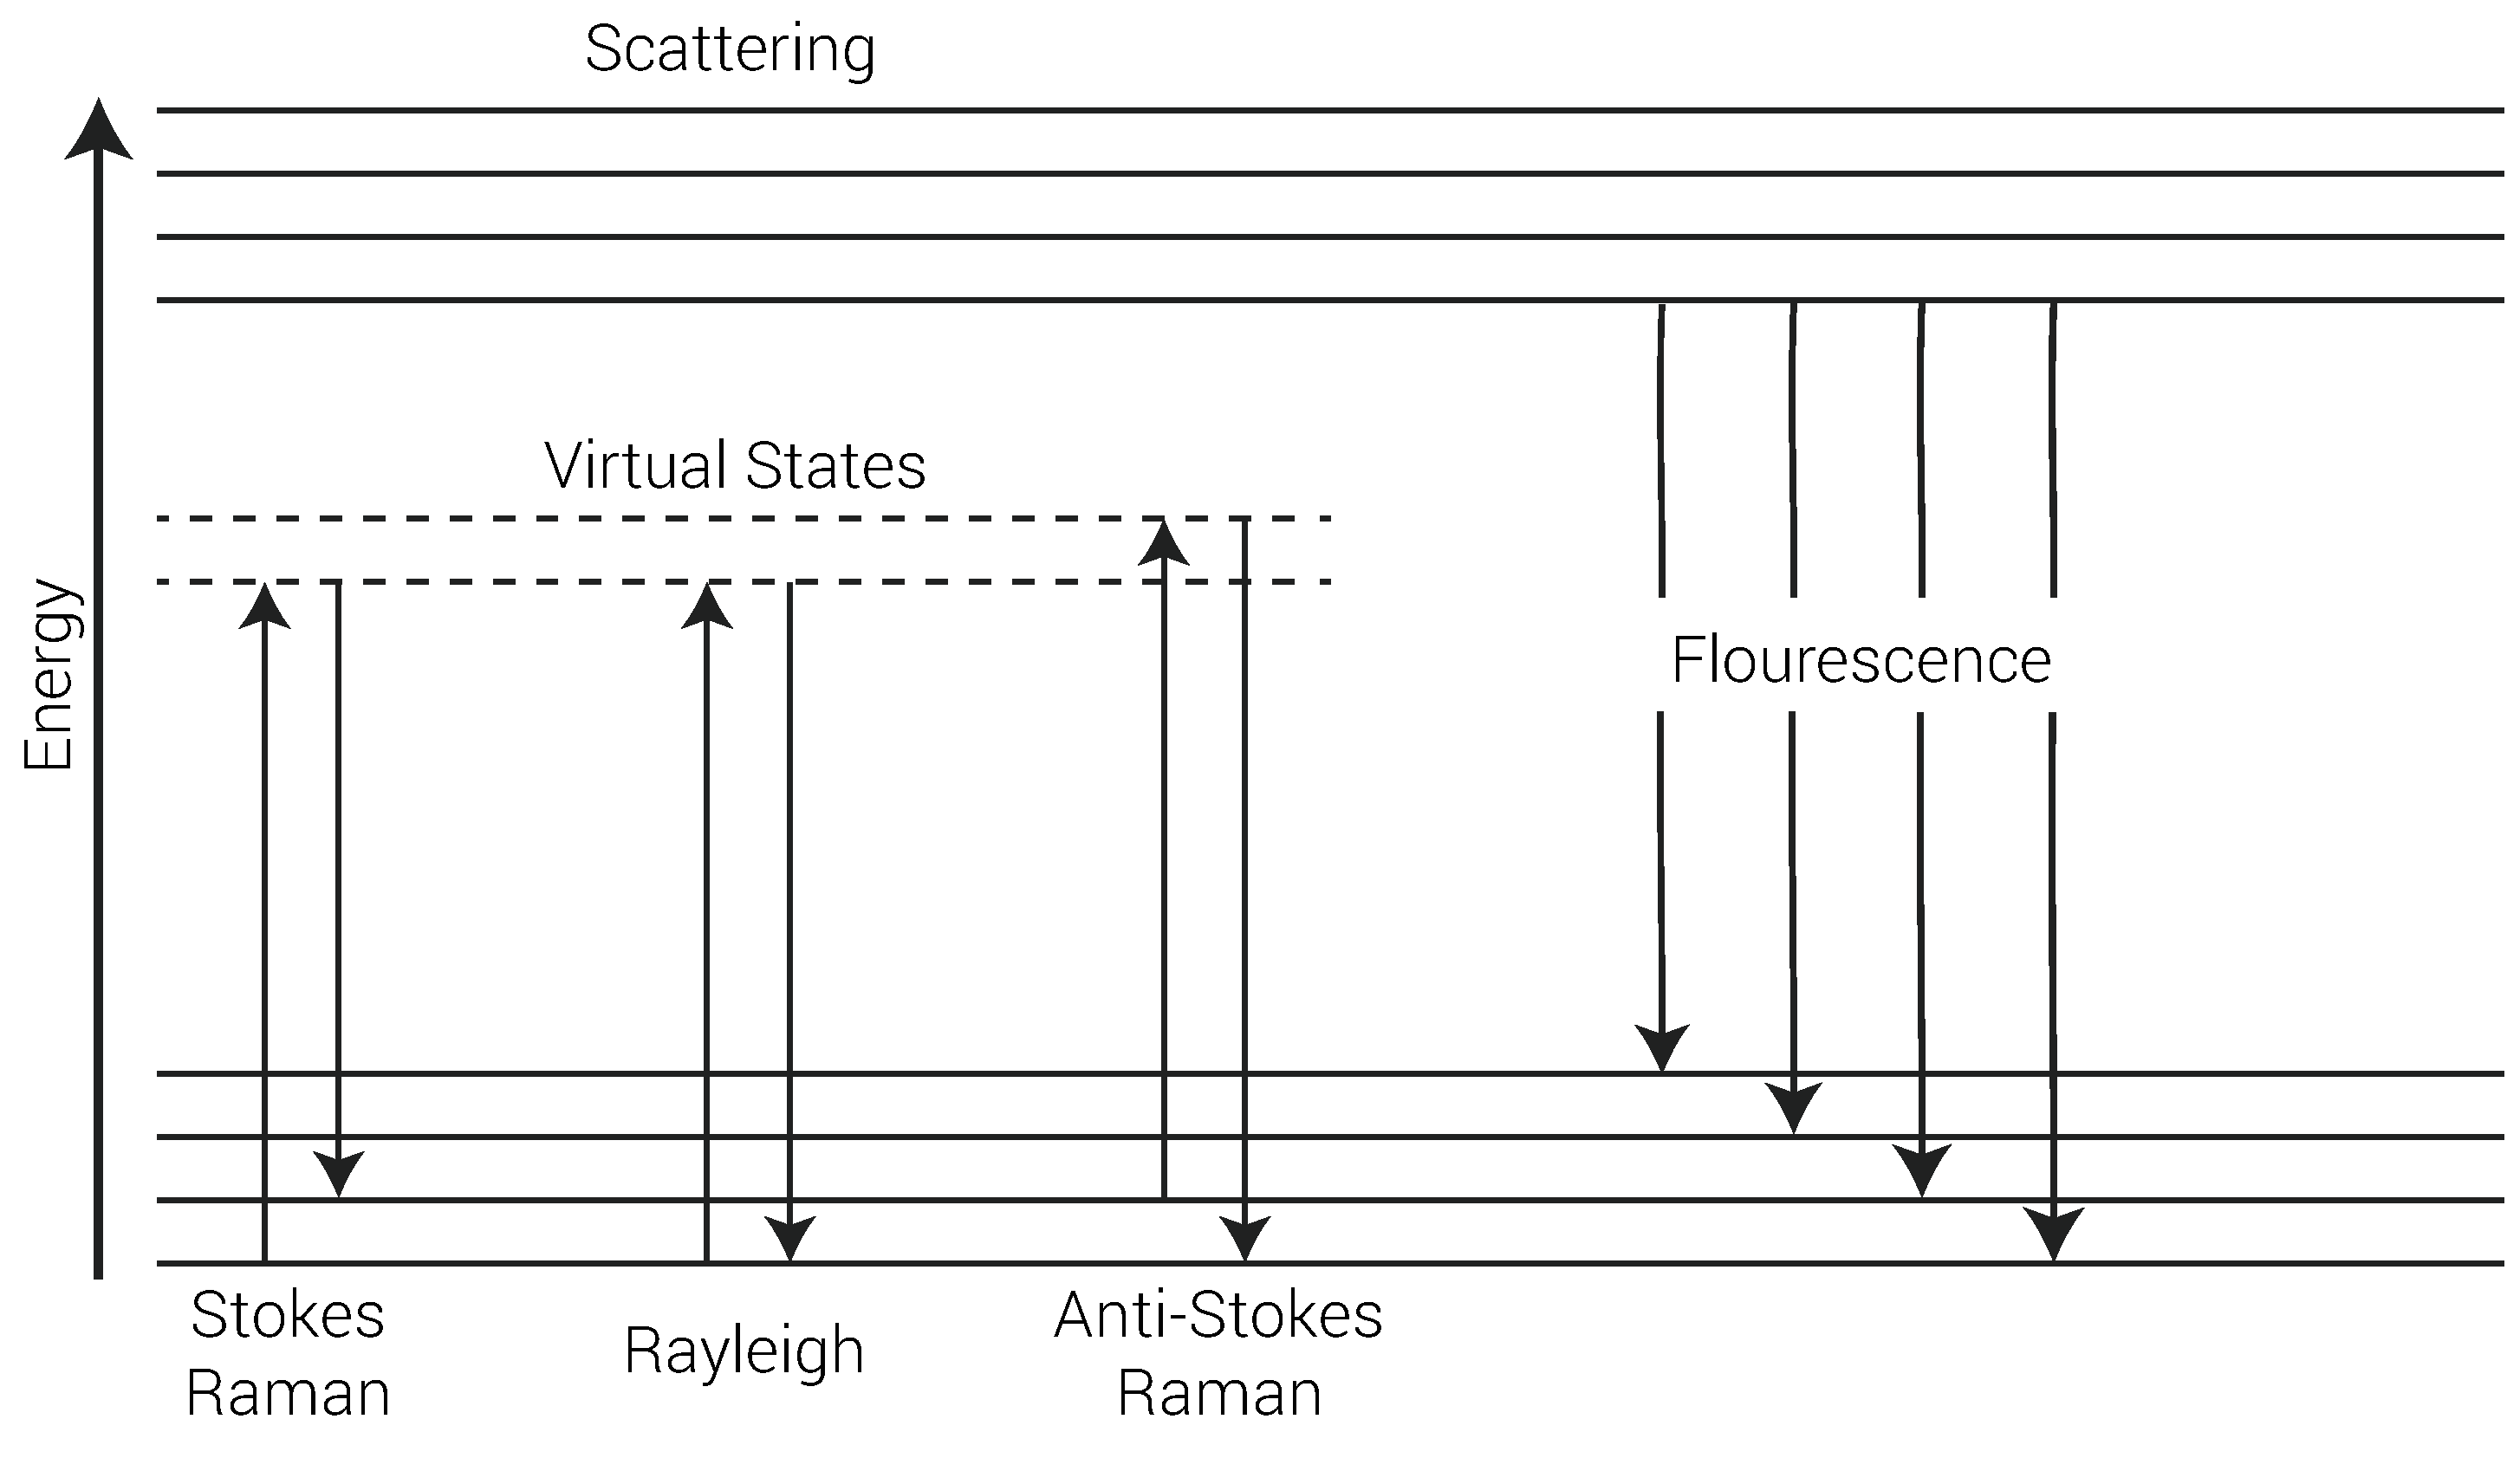
\includegraphics[width=0.7\linewidth]{raman_effect}
\caption{Diagram of the Raman effect. Horizontal lines represent energy levels of a system photons are incident upon, while vertical lines represent transitions between these levels. At right, the Raman effect is compared to fluorescence, which occurs when a system is excited to a high energy level and collapses to a lower one, emitting a photon in the process.}
\label{fig:raman_effect}
\end{figure}

This effect is illustrated graphically in Figure \ref{fig:raman_effect}. When, after being excited by a photon, a system returns to an energy level above its original state, the photon is re-emitted with a lower frequency; this is referred to as Stokes Raman radiation. The opposite effect, in which the system returns to a lower energy state than it started in, results in an increased-frequency photon and is referred to as Anti-Stokes Raman radiation.

It is important to note that the Raman effect operates on so-called ``virtual'' energy states. This nomenclature refers to short-lived states which are not full-fledged quantum states (solutions to the system Hamiltonian). They serve simply as intermediate states during the photon absorption and scattering process, and are generally considered to be more mathematical abstractions than physical entities \cite{RefWorks:31}.

To sum up; a molecule vibrates with distinct vibrational modes. Some of these modes affect the molecule's polarizability \textemdash these are referred to as Raman-active modes. As a result, light incident on the molecule may be shifted in frequency by the characteristic frequency of vibrational modes. Therefore the spectrum of reflected light will contain a peak for each Raman-active mode, with a frequency that reveals the vibration's $\nu_\mathrm{vib}$ and an intensity that reveals how strongly that vibration affects the polarizability. A generic example of such a spectrum is shown in figure \ref{fig:generic_spectrum}.

\begin{figure}
\centering
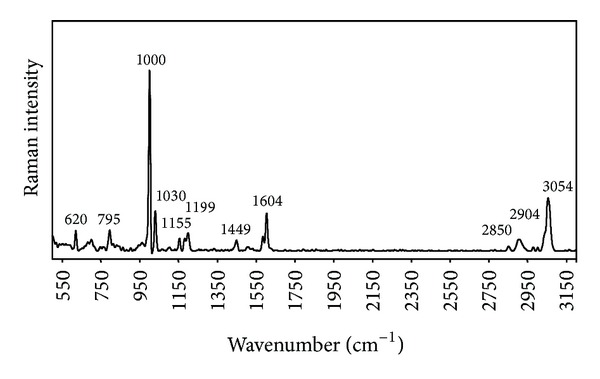
\includegraphics[width=0.7\linewidth]{generic_spectrum}
\caption{Raman spectrum of polystyrene fibers \cite{RefWorks:54}. Peaks indicate the frequency and intensity of Raman-shifted light.}
\label{fig:generic_spectrum}
\end{figure}

The Raman effect is observed generally with visible frequencies of incident light. However, if the incident frequency is decreased into the infrared region, a different effect is observed; infrared adsorption. This phenomenon is the basis of infrared (IR) spectroscopy.

Infrared light has a frequency in the range of $40-\SI{4,000}{cm^{-1}}$. Most molecular vibrational modes have a $\nu_\mathrm{vib}$ in the same range. This coincidence is what makes IR so useful, since IR light is precisely the right energy to excite the vibrational modes of molecules without scattering. When an IR photon in incident on a molecule, if its frequency is the same as that of one of the molecule's vibrational modes, the photon may be absorbed and excite that mode to a higher energy state. In contrast to the Raman effect, no photon is emitted at the end of this process. The result is an absorption, rather than scattering, spectrum; spectroscopists illuminate samples with a wide range of IR frequencies, and measure decreases in the intensity of transmitted light at the frequencies that match those of the sample's vibrational modes. An example of such a spectrum is shown in Figure \ref{fig:generic_ir}

\begin{figure}
\centering
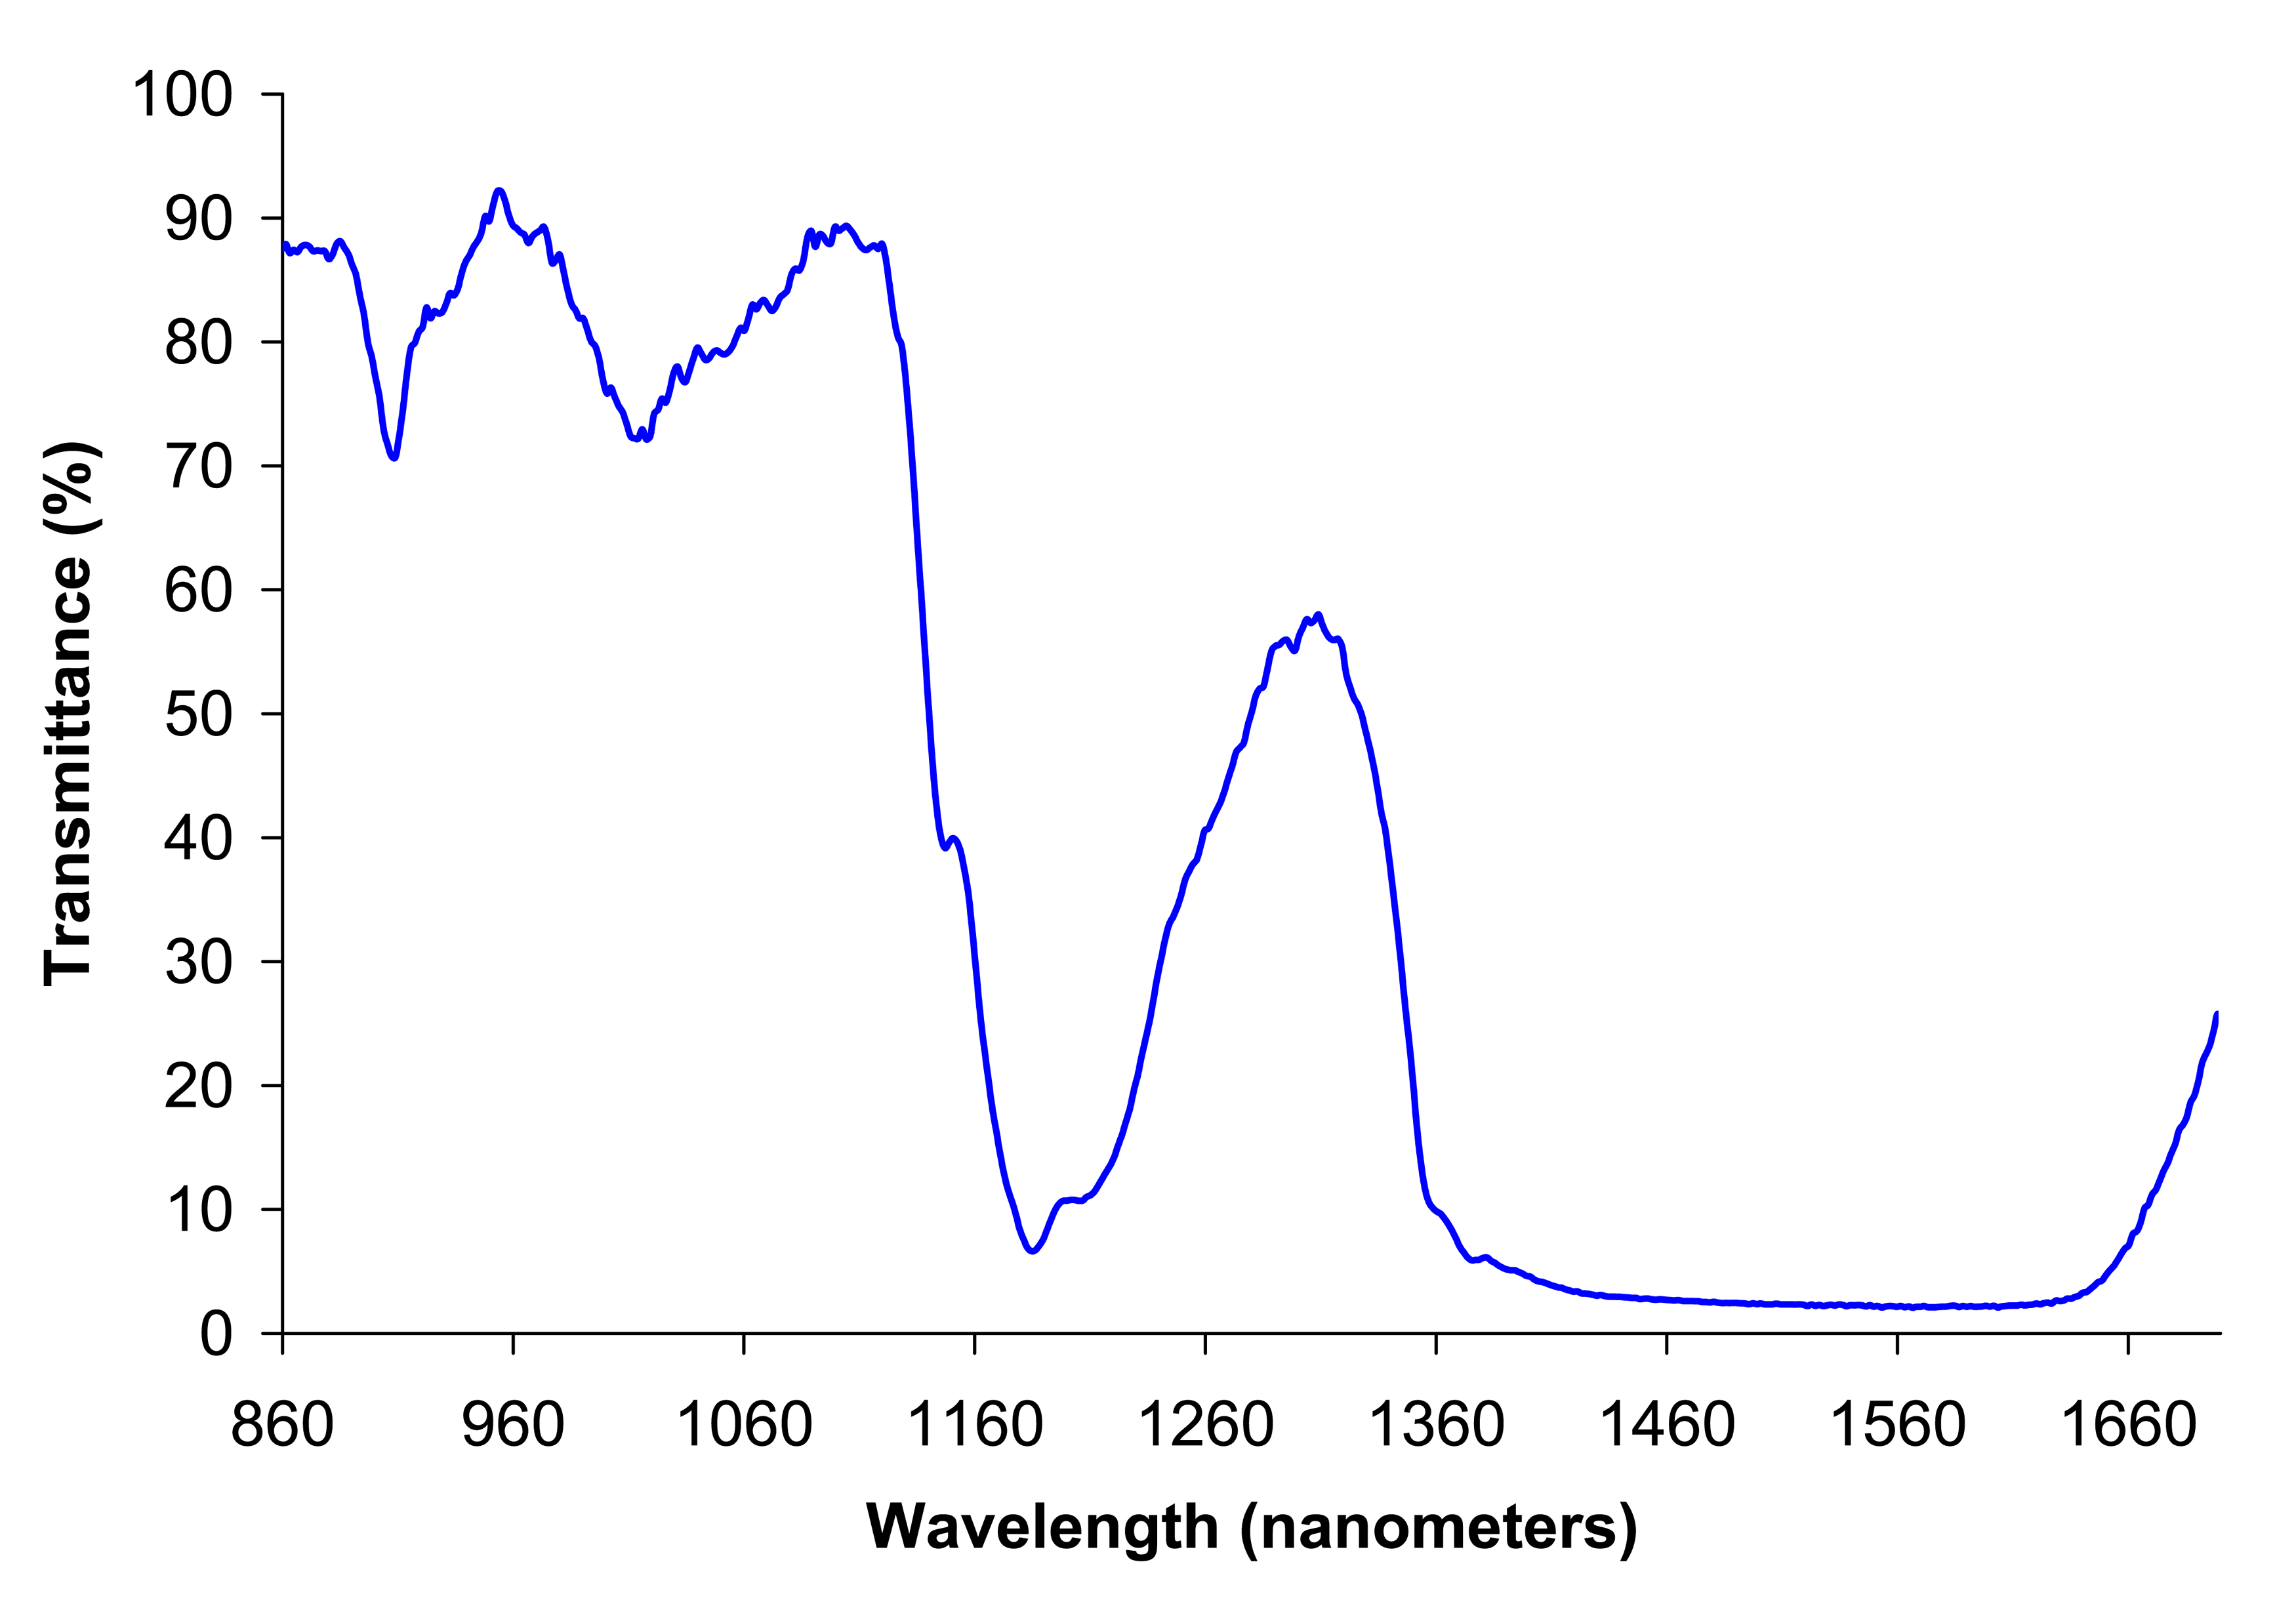
\includegraphics[width=0.8\linewidth]{generic_ir}
\caption{Generic IR spectrum, from Wikipedia. In contrast to Raman spectra, troughs are seen at vibrational frequencies, rather than peaks.}
\label{fig:generic_ir}
\end{figure}

There is one important restriction on IR adsorption as described here; vibrational modes can only be excited by IR photons if that vibration affects the molecule's dipole moment. In fact, analogously to how polarizability affects the intensity of Raman radiation, the extent to which a vibration affects a molecule's dipole moment dictates how strongly it will absorb incident photons. This restriction makes IR spectroscopy a perfect complement to the Raman variety, since many modes that are IR-active are not Raman-active, and vice versa. Deploying the two techniques in tandem thus allows a full vibrational picture of a material to be developed.

\section{Pyrolysis}

\begin{figure*}
	\centering
	\subfloat[Broido (1976) multistep model.]{
		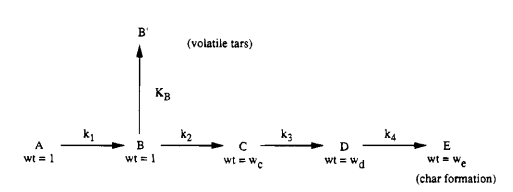
\includegraphics[width=.8\linewidth]{broido}
	}\\
	\subfloat[Bradbury, Sakai, and Shafizadeh (1979) active cellulose model.]{
		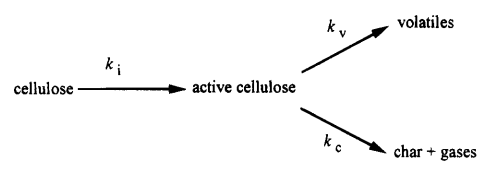
\includegraphics[width=.5\linewidth]{bradbury}
	}
	\subfloat[Varegyi et. al. (1993) high-pressure model.]{
		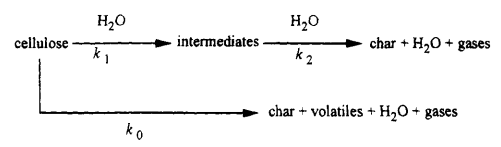
\includegraphics[width=.5\linewidth]{varhegyi}
	}
	\caption{Schematics of various proposed models for cellulose pyrolysis\cite{RefWorks:56}.}
	\label{fig:pyro_models}
\end{figure*}

Pyrolysis is defined as the thermal decomposition of materials in the absence of oxygen \cite{RefWorks:56}. In other words, this process involves breaking down materials without oxidizing them, as occurs during combustion. When this technique is applied to biomass, the result is typically a carbon and energy-rich substance, such as a solid char, an oil, or volatile gases. A familiar example of a pyrolytic process is the production of charcoal, which can be done by heating wood to approximately \SI{500}{\celsius} in a reduced-oxygen environment.

The wide spectrum of products created by biomass pyrolysis is one of its chief advantages as a method of biofuel production. Typically, pyrolyzed cellulose is converted to levoglucosan, glycolaldehyde and anhydrocellulose \cite{RefWorks:56, RefWorks:57}. These chemicals can be broken down further to produce a range of chemicals including furan, hydroxymethylfuran, furfural, tar, and fermentable sugars. Some of these can be processed into a variety of useful products, including ethanol, bio-oil, and other industrial feedstocks. The wide range of pyrolysis products suggests that cellulose could form the basic renewable precursor for a whole host of widely used chemicals, which would make it invaluable in a post-fossil-fuel world.

The distribution of products from cellulose pyrolysis can be coarsely controlled by means of varying the duration of the reaction, the rate of heating, and the presence/concentration of additives such as inorganic salts \cite{RefWorks:59}. However, these techniques are still crude due to our incomplete understanding of how pyrolysis actually occurs in cellulose. Many models of this process have been proposed over the past few decades, several of which can be seen in schematic form in Figure \ref{fig:pyro_models} \cite{RefWorks:58}. These models typically take the form of an initiation step followed by one or more competitive reaction pathways. In some cases, this initiation step involves a transition to a poorly defined state known as ``active cellulose,'' from which further degradation occurs.

\begin{figure}
	\centering
	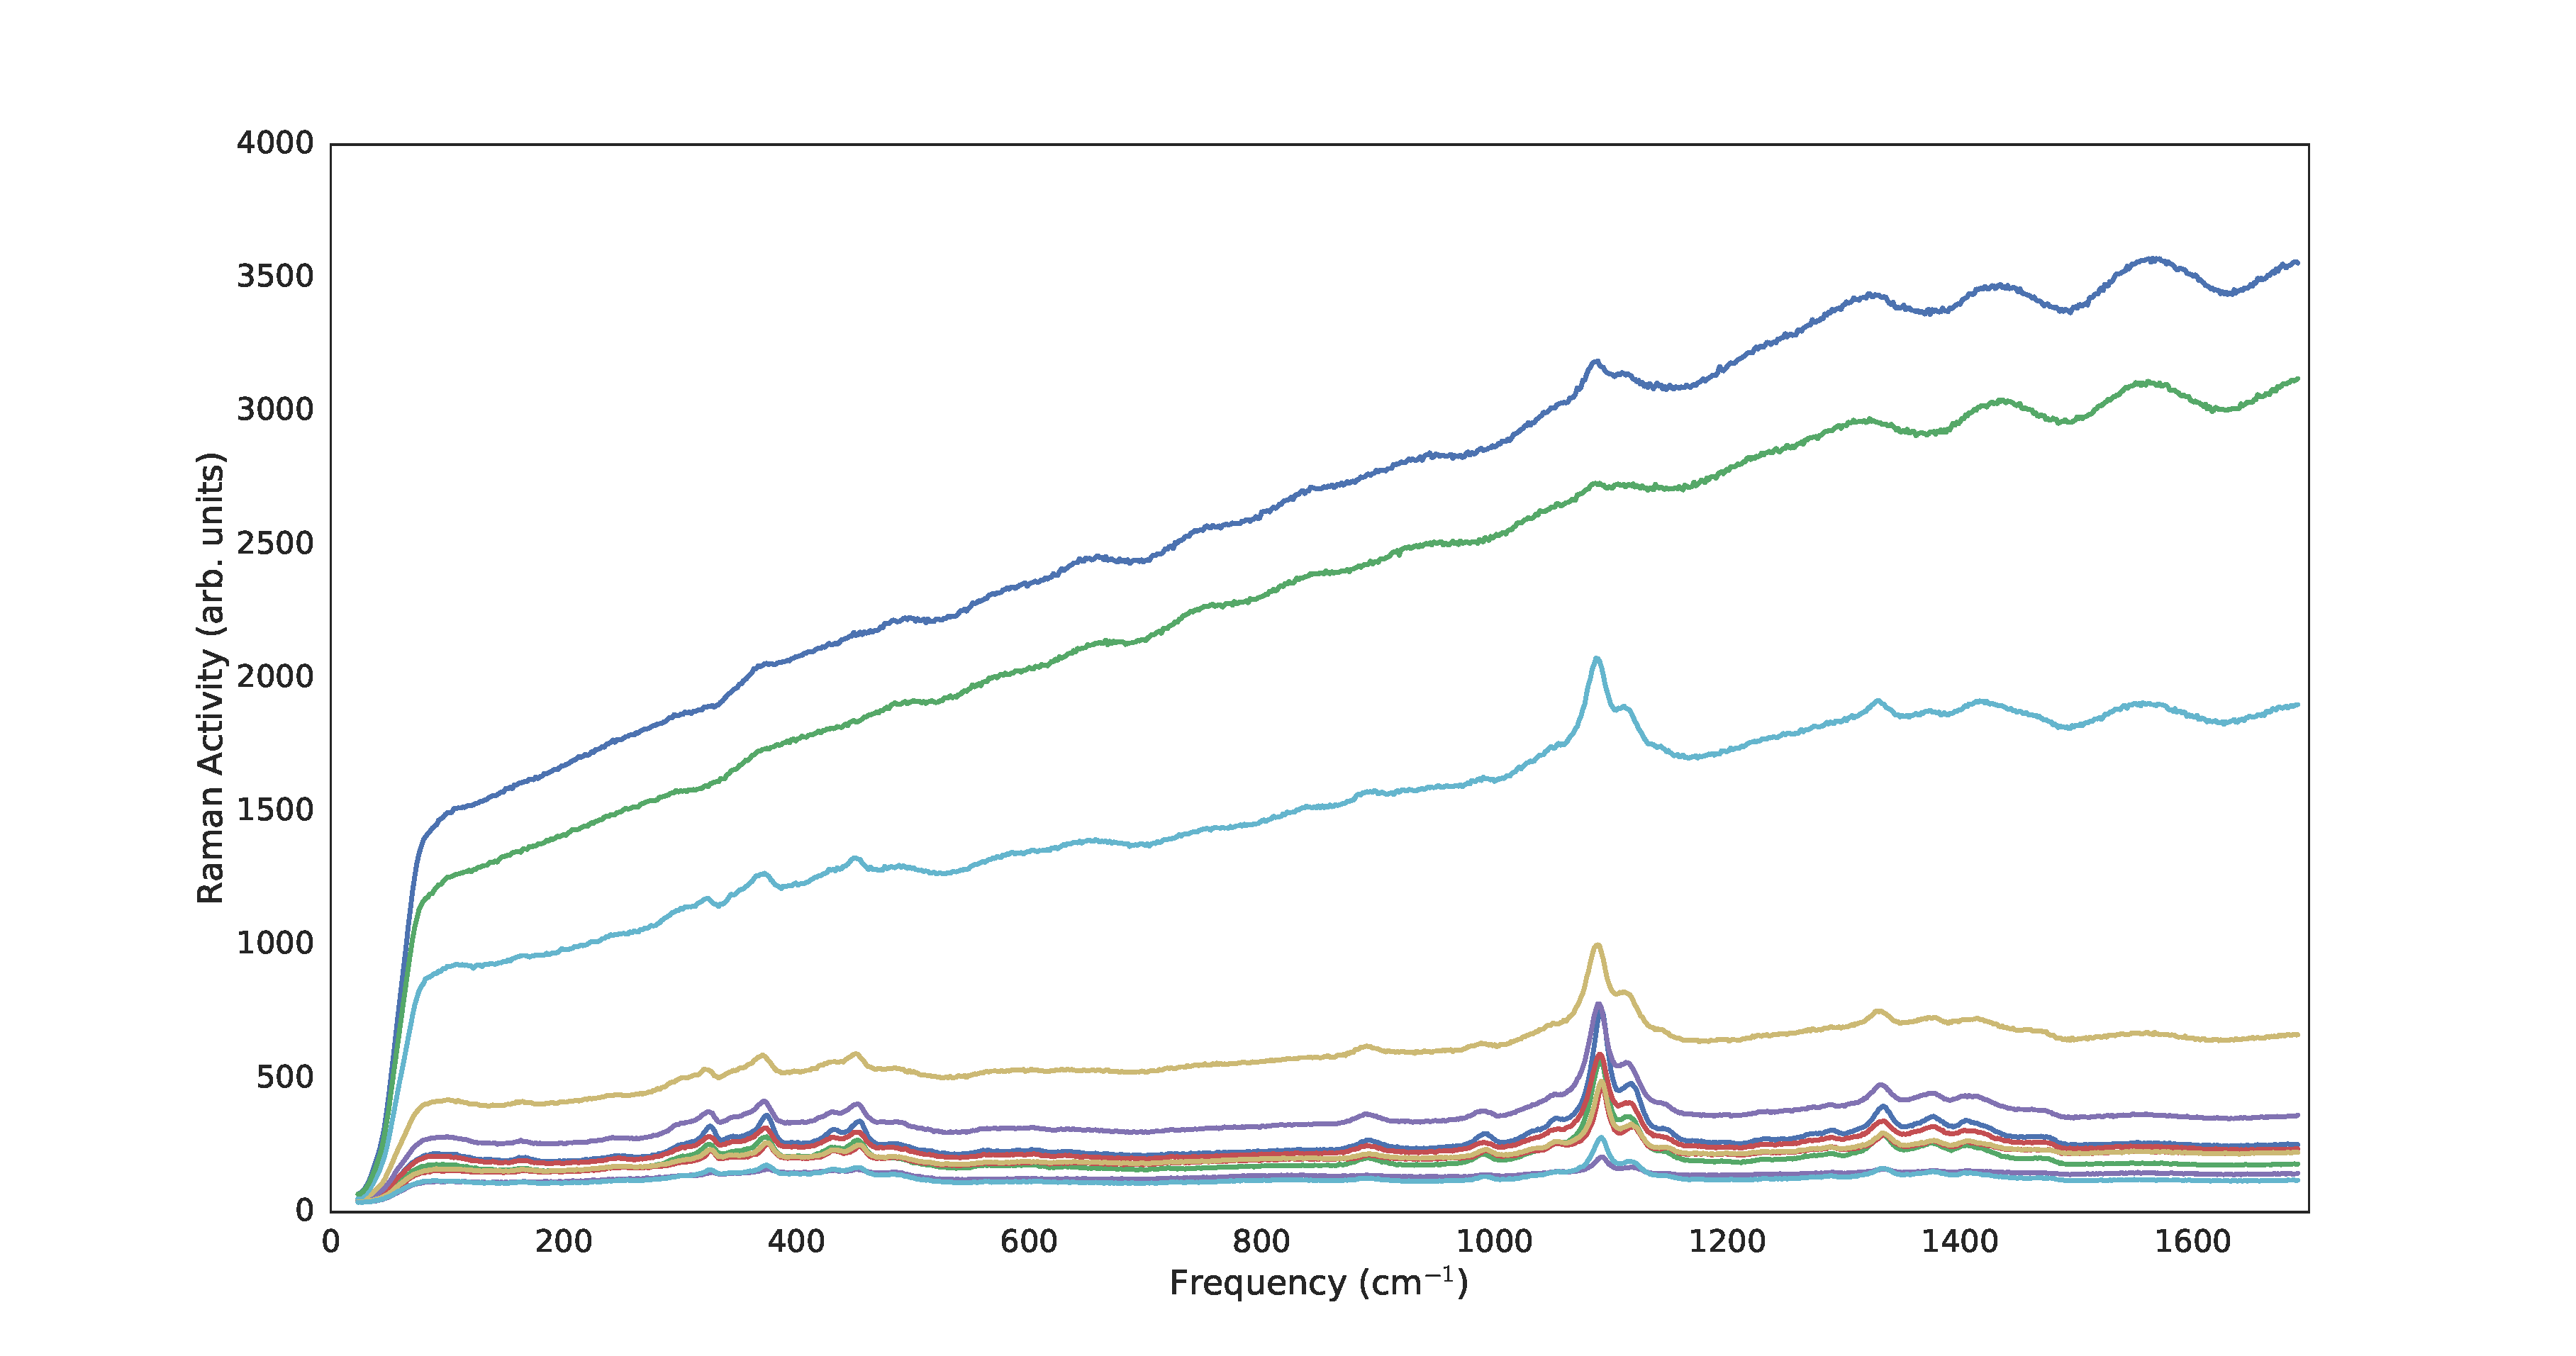
\includegraphics[width=\linewidth]{ref_plot}
	\caption{Raman spectrum of cellulose at different temperatures. Data courtesy of Michael Timko and Geoffrey Tompsett, Worcester Polytechnical Institute.}
	\label{fig:ref_plot}
\end{figure}

A primary goal of the present work is to gain insight into the onset of pyrolysis, including how it begins and at what temperature this occurs. Past research has indicated that pyrolysis is initiated at temperature ranging from 250\textendash400 \si{\celsius} (523-673 K)\cite{RefWorks:58}. However, recent work at Worcester Polytechnical Institute led by Mike Timko and Geoffrey Tompsett has shown that the Raman spectrum of cellulose actually starts to change dramatically at temperatures as low as 473K, shown in Figure \ref{fig:ref_plot}. This change may indicate heretofore unobserved chemical or structural changes being caused by heating. Identifying the causes of this change is another goal of this thesis. We aim to do this by developing an effective method for simulating the vibrational behavior and thus the Raman spectrum of cellulose at different temperatures. With this model in hand, we can then answer the question, ``what causes the Raman spectrum of cellulose to change at 483K?'' By answering this question, we will come  a bit closer to answering an even more important question: ``how do we make biofuels more efficiently?''
